\documentclass[conference]{IEEEtran}

\usepackage{cite}
\usepackage{graphicx}
\usepackage{booktabs}
\usepackage[caption=false,font=footnotesize]{subfig}
\usepackage{url}

\title{KMNIST Handwriting Recognition Using a Simple Convolutional Neural Network in PyTorch}
\author{
\IEEEauthorblockN{Family-5.3-Plus Group}
\IEEEauthorblockA{
The School of Data Science, Lingnan University\\
Repository: \url{https://github.com/Lil3bear/CDS525_Group_Project.git}\\
Team members and contribution statement are listed in Appendix A.
}
}

\begin{document}

\maketitle

\begin{abstract}
This paper presents a completed KMNIST handwriting-recognition project implemented in PyTorch using a compact convolutional neural network. The goal was to produce a strong, reproducible coursework submission with a model that remains easy to explain and efficient to train. The final system includes local dataset loading, preprocessing, validation-based checkpointing, metric logging, experiment automation, figure generation, and qualitative prediction visualization. The baseline configuration uses cross-entropy loss, the Adam optimizer, learning rate 0.001, batch size 64, and 12 epochs, achieving a best validation accuracy of 98.60\% and a best test accuracy of 95.63\%. Additional experiments compare an alternate label-smoothed loss, four learning rates, and five batch sizes using the saved outputs generated by the project. The alternate loss improves final test accuracy to 96.40\%, the learning-rate sweep shows that 0.001 is the most effective value among the tested settings, and the batch-size sweep indicates relatively limited sensitivity compared with learning rate. The results show that a small CNN can achieve strong KMNIST performance while supporting clear analysis and reproducible reporting in an academic project setting.
\end{abstract}

\begin{IEEEkeywords}
KMNIST, handwriting recognition, convolutional neural network, PyTorch, hyperparameter tuning, image classification
\end{IEEEkeywords}

\section{Introduction}

Handwriting recognition remains a useful benchmark problem in machine learning and computer vision because it combines image processing, feature learning, and multi-class classification in a form that is relatively easy to interpret. For university coursework, it is especially suitable because the task is complex enough to demonstrate the main stages of a deep learning pipeline, but compact enough to be implemented, trained, and analyzed within limited time and computing resources. A successful solution must convert images into a suitable tensor representation, learn visual features that discriminate between similar classes, optimize model parameters effectively, and produce results that generalize beyond the training set.

This report presents a completed deep learning project on KMNIST, a dataset of 10 classes of handwritten Kuzushiji characters introduced as a more challenging alternative to the standard MNIST benchmark \cite{clanuwat2018}. Unlike decimal digits, Kuzushiji characters often contain stroke patterns that are visually similar across classes, so strong classification performance requires the model to capture fine local structure rather than relying on obvious global differences. Each KMNIST image is a grayscale image of size $28 \times 28$, which makes the dataset computationally manageable while still being non-trivial for classification.

The objective of the project was to produce a high-quality university submission using a model and workflow that remain easy to explain, reproduce, and defend. Instead of pursuing unnecessary architectural complexity, the implementation favors a compact convolutional neural network (CNN) in PyTorch \cite{paszke2019} together with a small number of targeted experimental comparisons. This decision reflects an important practical consideration in academic project work: strong performance is valuable, but so are clarity of design, sound justification of modeling choices, and the ability to communicate the full system clearly in a written report and oral presentation.

The completed repository includes the full workflow needed for a submission-ready project. The code handles data loading, preprocessing, model definition, training, validation, testing, checkpoint saving, metric logging, plotting, and qualitative visualization of predictions. The project also includes comparison experiments for an alternate loss function, a learning-rate sweep over the required values $\{0.1, 0.01, 0.001, 0.0001\}$, and a batch-size sweep over the required values $\{8, 16, 32, 64, 128\}$. The figures used in this report are the actual outputs generated by those completed runs, not reconstructed or hypothetical illustrations.

Within this repository, the KMNIST data are stored locally as NumPy files in \texttt{data/KMNIST/npz}. A direct inspection of the saved arrays shows that the project uses 60{,}000 training images and 10{,}000 test images, together with their corresponding labels. The availability of local arrays keeps the workflow stable inside the project environment and avoids any dependence on external downloads at report-writing time. The learning problem itself remains the same: the model must assign each grayscale character image to one of 10 classes.

The central research question of this work is straightforward: can a small CNN, trained with a clear and reproducible PyTorch pipeline, achieve strong KMNIST recognition accuracy while also supporting the hyperparameter analysis and performance visualization required by the assignment? The completed results show that it can. The baseline model achieved a best test accuracy of $95.63\%$, while the alternate label-smoothed loss achieved $96.40\%$. At the same time, the model and training code remain short enough to be understood and explained by students without relying on advanced engineering features.

The remainder of this report is organized as follows. Section 2 explains the design of the system, including the preprocessing pipeline, train/validation/test setup, CNN architecture, loss function, optimizer, and main hyperparameter choices. Section 3 presents the completed experimental results using the saved figures and summary files from the repository, covering the baseline model, the alternate loss comparison, the learning-rate sweep, the batch-size sweep, and the qualitative prediction visualization. Section 4 concludes with the main findings, limitations, and realistic directions for future improvement.

\section{Design \& Functions}

The project is organized into a small number of clearly separated Python files. This structure is intentionally simple because a coursework submission should be easy to inspect and explain. The file \texttt{data.py} is responsible for loading the KMNIST arrays, converting them into tensors, and creating the data loaders. The file \texttt{model.py} defines the CNN. The file \texttt{train.py} manages the training loop, validation loop, test evaluation, checkpoint saving, and metrics export. The file \texttt{experiments.py} runs the required comparisons for different loss functions, learning rates, and batch sizes. The file \texttt{plots.py} generates the final figure files from the saved CSV results, while \texttt{visualize\_predictions.py} produces the grid of the first 100 test predictions. This decomposition gives each file a single clear purpose and reduces the risk of hidden behavior in the workflow.

\subsection{Dataset preparation and preprocessing}

The raw project data are stored in four NumPy files: training images, training labels, test images, and test labels. The training image array has shape $(60000, 28, 28)$ and the test image array has shape $(10000, 28, 28)$, with unsigned 8-bit integer pixel values. During loading, the images are converted to floating-point tensors and reshaped into $(N, 1, 28, 28)$ so that the CNN receives a single grayscale channel as input. Labels are converted to integer tensors suitable for multi-class classification.

The preprocessing applied in \texttt{data.py} is intentionally modest. If image values exceed 1.0, they are scaled from the original $[0, 255]$ range into $[0, 1]$ by division by 255. After this, the images are normalized using mean $0.5$ and standard deviation $0.5$, which maps the inputs approximately into the range $[-1, 1]$. This is a standard preprocessing choice for small grayscale image datasets and helps the optimizer operate on a consistent numeric scale \cite{goodfellow2016}. No additional hand-crafted feature engineering is used, which keeps the data pipeline simple and reproducible.

The project uses a train/validation/test setup. The 60{,}000-image training portion of KMNIST is split into 54{,}000 training samples and 6{,}000 validation samples by using a fixed validation fraction of 0.1. The separate 10{,}000-image test set remains untouched during model selection. This is an appropriate evaluation design because validation accuracy is used to determine the best checkpoint during training, while test accuracy is reserved for reporting final generalization performance. The split is generated with a fixed seed of 42, which means repeated runs use the same data partition and therefore remain comparable.

\subsection{CNN architecture}

The classifier is a compact convolutional neural network defined in \texttt{model.py}. Its architecture contains two convolutional blocks followed by a small fully connected classifier:

\begin{itemize}
    \item \texttt{Conv2d(1, 32, kernel\_size=3, padding=1)}
    \item ReLU activation
    \item \texttt{MaxPool2d(kernel\_size=2)}
    \item \texttt{Conv2d(32, 64, kernel\_size=3, padding=1)}
    \item ReLU activation
    \item \texttt{MaxPool2d(kernel\_size=2)}
    \item Flatten
    \item \texttt{Linear(64 * 7 * 7, 128)}
    \item ReLU activation
    \item Dropout with probability 0.25
    \item \texttt{Linear(128, 10)}
\end{itemize}

This design is suitable for handwriting recognition because convolutional layers are effective at learning local patterns such as edges, curves, and stroke intersections \cite{lecun1998}. The first convolutional layer learns low-level visual patterns, while the second layer combines those local patterns into more discriminative higher-level features. Max pooling reduces the spatial resolution and helps the model focus on salient structure rather than exact pixel positions. The fully connected layers then combine the extracted feature maps into logits for the 10 output classes.

The architecture is intentionally small. For a dataset of $28 \times 28$ grayscale images, an extremely deep model would add complexity without being necessary for a strong assignment result. The chosen CNN provides a better balance between representational power and interpretability. It is clearly more appropriate for image classification than a purely fully connected network, yet still simple enough to describe line by line in a presentation.

\subsection{Loss function, optimizer, and hyperparameters}

The main baseline uses cross-entropy loss, implemented as \texttt{CrossEntropyLoss}. This is the standard choice for single-label multi-class classification because each image belongs to exactly one class and the network outputs one logit per class \cite{goodfellow2016}. Cross-entropy directly penalizes incorrect class probability assignments and therefore provides a natural objective for handwritten character recognition.

The alternate loss comparison uses \texttt{CrossEntropyLoss(label\_smoothing=0.1)}. Label smoothing was included because it is a lightweight regularization technique that can reduce overconfident predictions and sometimes improve generalization \cite{szegedy2016}. Importantly, this comparison changes only the loss configuration while keeping the architecture and remaining training setup fixed, making the experimental contrast easy to interpret.

The optimizer for all completed runs is Adam \cite{kingma2015}. Adam is a sensible choice for coursework because it converges quickly, is relatively stable under default settings, and usually requires less manual tuning than plain stochastic gradient descent. The saved experiment summaries show that the baseline configuration used a learning rate of 0.001, a batch size of 64, and 12 epochs. Those completed runs were executed on CPU, which is also informative: the model is light enough that the full experiment suite can be completed even without GPU hardware.

These hyperparameters were selected for practical reasons. A learning rate of 0.001 is a widely used starting point for Adam and, as shown later in the experiments, it was the best-performing value among the required learning-rate choices. A batch size of 64 is large enough to give stable updates while remaining computationally manageable. Twelve epochs are sufficient to show clear learning curves and convergence trends without making the experiment suite excessively long. Collectively, these choices create a training setup that is both academically defensible and operationally efficient.

\subsection{Training workflow and saved outputs}

The training workflow implemented in \texttt{train.py} records training loss, training accuracy, validation loss, validation accuracy, test loss, and test accuracy at every epoch. After each epoch, the model checkpoint is updated whenever validation accuracy improves. This is a sound procedure because it bases model selection on validation data rather than directly on the test set.

For each run, the repository stores three key outputs: a CSV file of per-epoch metrics in the \texttt{results} directory, a summary configuration file in JSON format, and a best-model checkpoint in the \texttt{checkpoints} directory. The plotting script then reads the saved CSV files and generates the final PNG figures used in this report. As a result, the numerical analysis and the visual analysis are both tied directly to saved artifacts from the completed experiments rather than to undocumented console output.

From a software-engineering perspective, this workflow is one of the strengths of the project. The code is organized, the outputs are traceable, and the experimental pipeline can be re-run in a straightforward way. From an academic perspective, that organization improves credibility because every major claim in the report can be linked back to a saved result file or figure.

\section{Demonstration \& Performance}

This section reports the completed experimental findings using the saved metrics and figures already present in the repository. The analysis focuses on the baseline model, the alternate loss comparison, the learning-rate sweep, the batch-size sweep, and the qualitative visualization of the first 100 test predictions.

\subsection{Baseline model performance}

The baseline run uses cross-entropy loss, Adam with learning rate 0.001, batch size 64, and 12 training epochs. Its learning curves are shown in Figure~\ref{fig:baseline_curves}. The training behavior is stable and easy to interpret. Training loss decreases from 0.3538 in the first epoch to 0.0163 in the final epoch, while training accuracy rises from $89.01\%$ to $99.48\%$. This indicates that the CNN has more than enough capacity to fit the training data.

More importantly, the model generalizes well. The best validation accuracy reached $98.60\%$ at epoch 10. The best test accuracy observed during training was $95.63\%$, and the final test accuracy at epoch 12 was $95.59\%$. The small difference between the best and final test accuracy suggests that the model remained stable near the end of training. There is some expected gap between training and test performance, but the overall generalization level is high for such a compact architecture.

\begin{figure*}[!t]
    \centering
    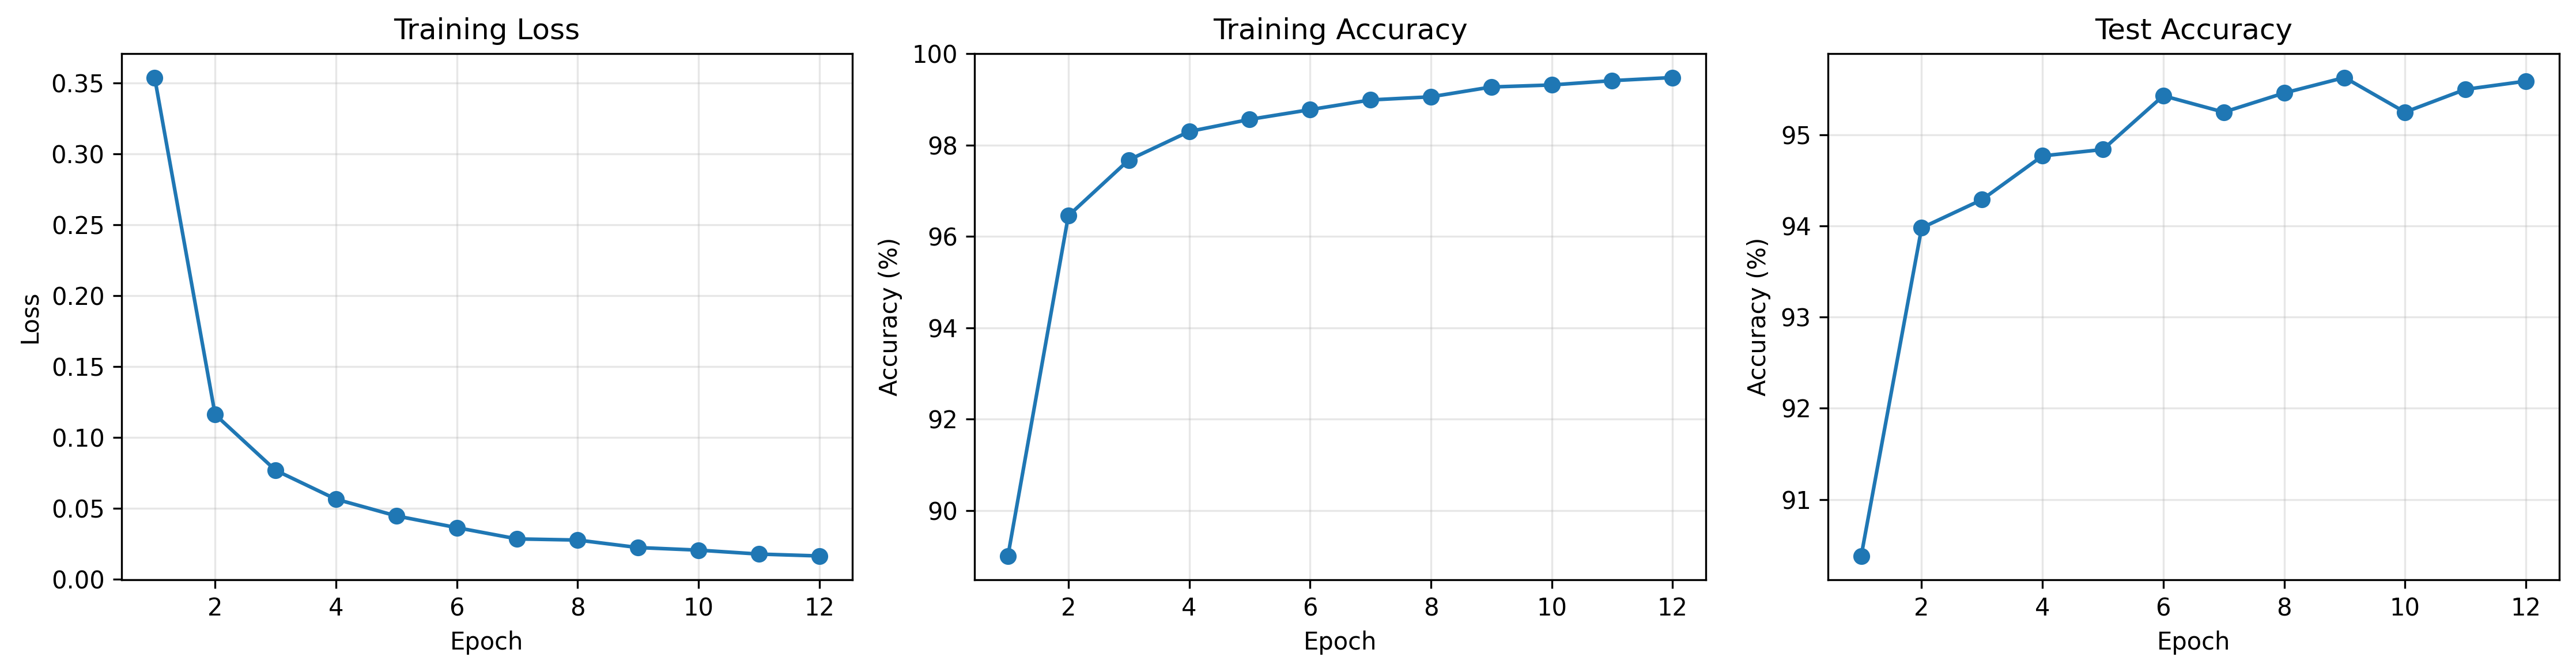
\includegraphics[width=0.98\textwidth,keepaspectratio]{figures/baseline_training_curves.png}
    \caption{Baseline training curves for the main CNN, showing training loss, training accuracy, and test accuracy over 12 epochs.}
    \label{fig:baseline_curves}
\end{figure*}

\begin{table}[t]
    \centering
    \scriptsize
    \resizebox{\columnwidth}{!}{%
    \begin{tabular}{lcccc}
        \toprule
        Run & Best epoch & Best validation acc. & Best test acc. & Final test acc. \\
        \midrule
        Baseline cross-entropy & 10 & 98.60\% & 95.63\% & 95.59\% \\
        Label-smoothed loss & 10 & 98.92\% & 96.40\% & 96.40\% \\
        \bottomrule
    \end{tabular}
    }
    \caption{Summary of the baseline run and the alternate loss comparison using the saved experiment summaries.}
    \label{tab:baseline_loss}
\end{table}

As a baseline for the rest of the study, these results are strong. They show that a straightforward CNN can already solve KMNIST at a high level of accuracy without requiring a deeper architecture, extensive regularization, or complex training schedules. That makes the baseline a credible reference point for the remaining experiments.

\subsection{Comparison with an alternate loss function}

The assignment required a comparison using a different loss function. In this project, the baseline \texttt{CrossEntropyLoss} was compared with a label-smoothed variant, \texttt{CrossEntropyLoss(label\_smoothing=0.1)}. The comparison is shown in Figure~\ref{fig:loss_comparison}, and the key numerical results are summarized in Table~\ref{tab:baseline_loss}.

This experiment is methodologically clean because all other factors are unchanged: the network architecture, optimizer, learning rate, batch size, epoch count, validation split, and random seed are the same. The only difference is the form of the loss function. Under these conditions, the label-smoothed model achieved a best validation accuracy of $98.92\%$, a best test accuracy of $96.40\%$, and a final test accuracy of $96.40\%$. Relative to the baseline, the final test accuracy improved by 0.81 percentage points.

Although the gain is modest, it is meaningful. The result suggests that the baseline network benefits from a small amount of output regularization. A plausible explanation is that label smoothing reduces excessive confidence in the predicted class distribution and encourages slightly better generalization on unseen samples \cite{szegedy2016}. This is an important finding because it shows that improvement does not necessarily require a larger model; in this case, a minor change to the loss function was enough to produce better test performance.

\begin{figure*}[!t]
    \centering
    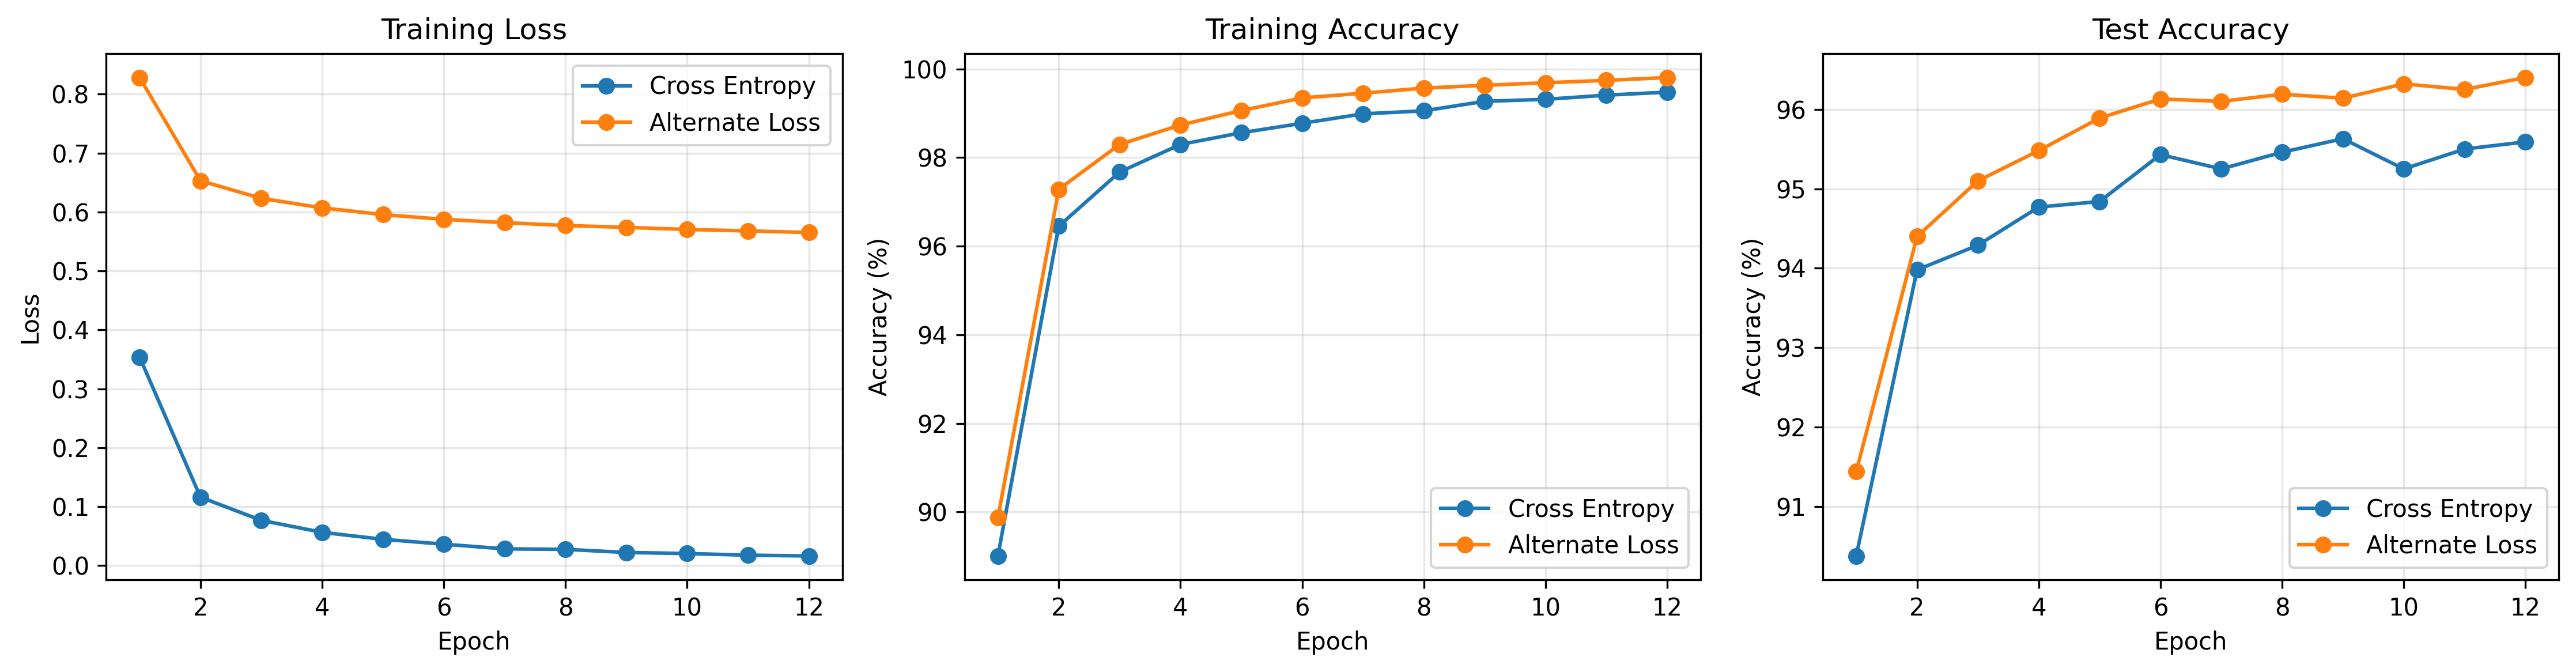
\includegraphics[width=0.98\textwidth,keepaspectratio]{figures/loss_comparison.png}
    \caption{Comparison between the baseline cross-entropy loss and label-smoothed cross-entropy. The figure reports training loss, training accuracy, and test accuracy across epochs.}
    \label{fig:loss_comparison}
\end{figure*}

At the same time, the baseline cross-entropy configuration remains important. It is simpler to explain, widely used in introductory classification tasks, and already produces strong results. Therefore, the alternate loss should be interpreted as a useful improvement rather than as evidence that the original baseline was poorly chosen.

\subsection{Learning-rate comparison}

The learning-rate sweep is one of the most informative parts of the project because it shows how strongly optimization quality depends on this hyperparameter. The tested values were 0.1, 0.01, 0.001, and 0.0001, all with the same architecture, optimizer, batch size, epoch count, and loss function. The corresponding training-loss and accuracy figures are shown in Figure~\ref{fig:lr_comparison}, and the summary values are listed in Table~\ref{tab:lr_sweep}.

\begin{figure*}[!t]
    \centering
    \subfloat[Training loss across learning rates.\label{fig:lr_loss}]{
        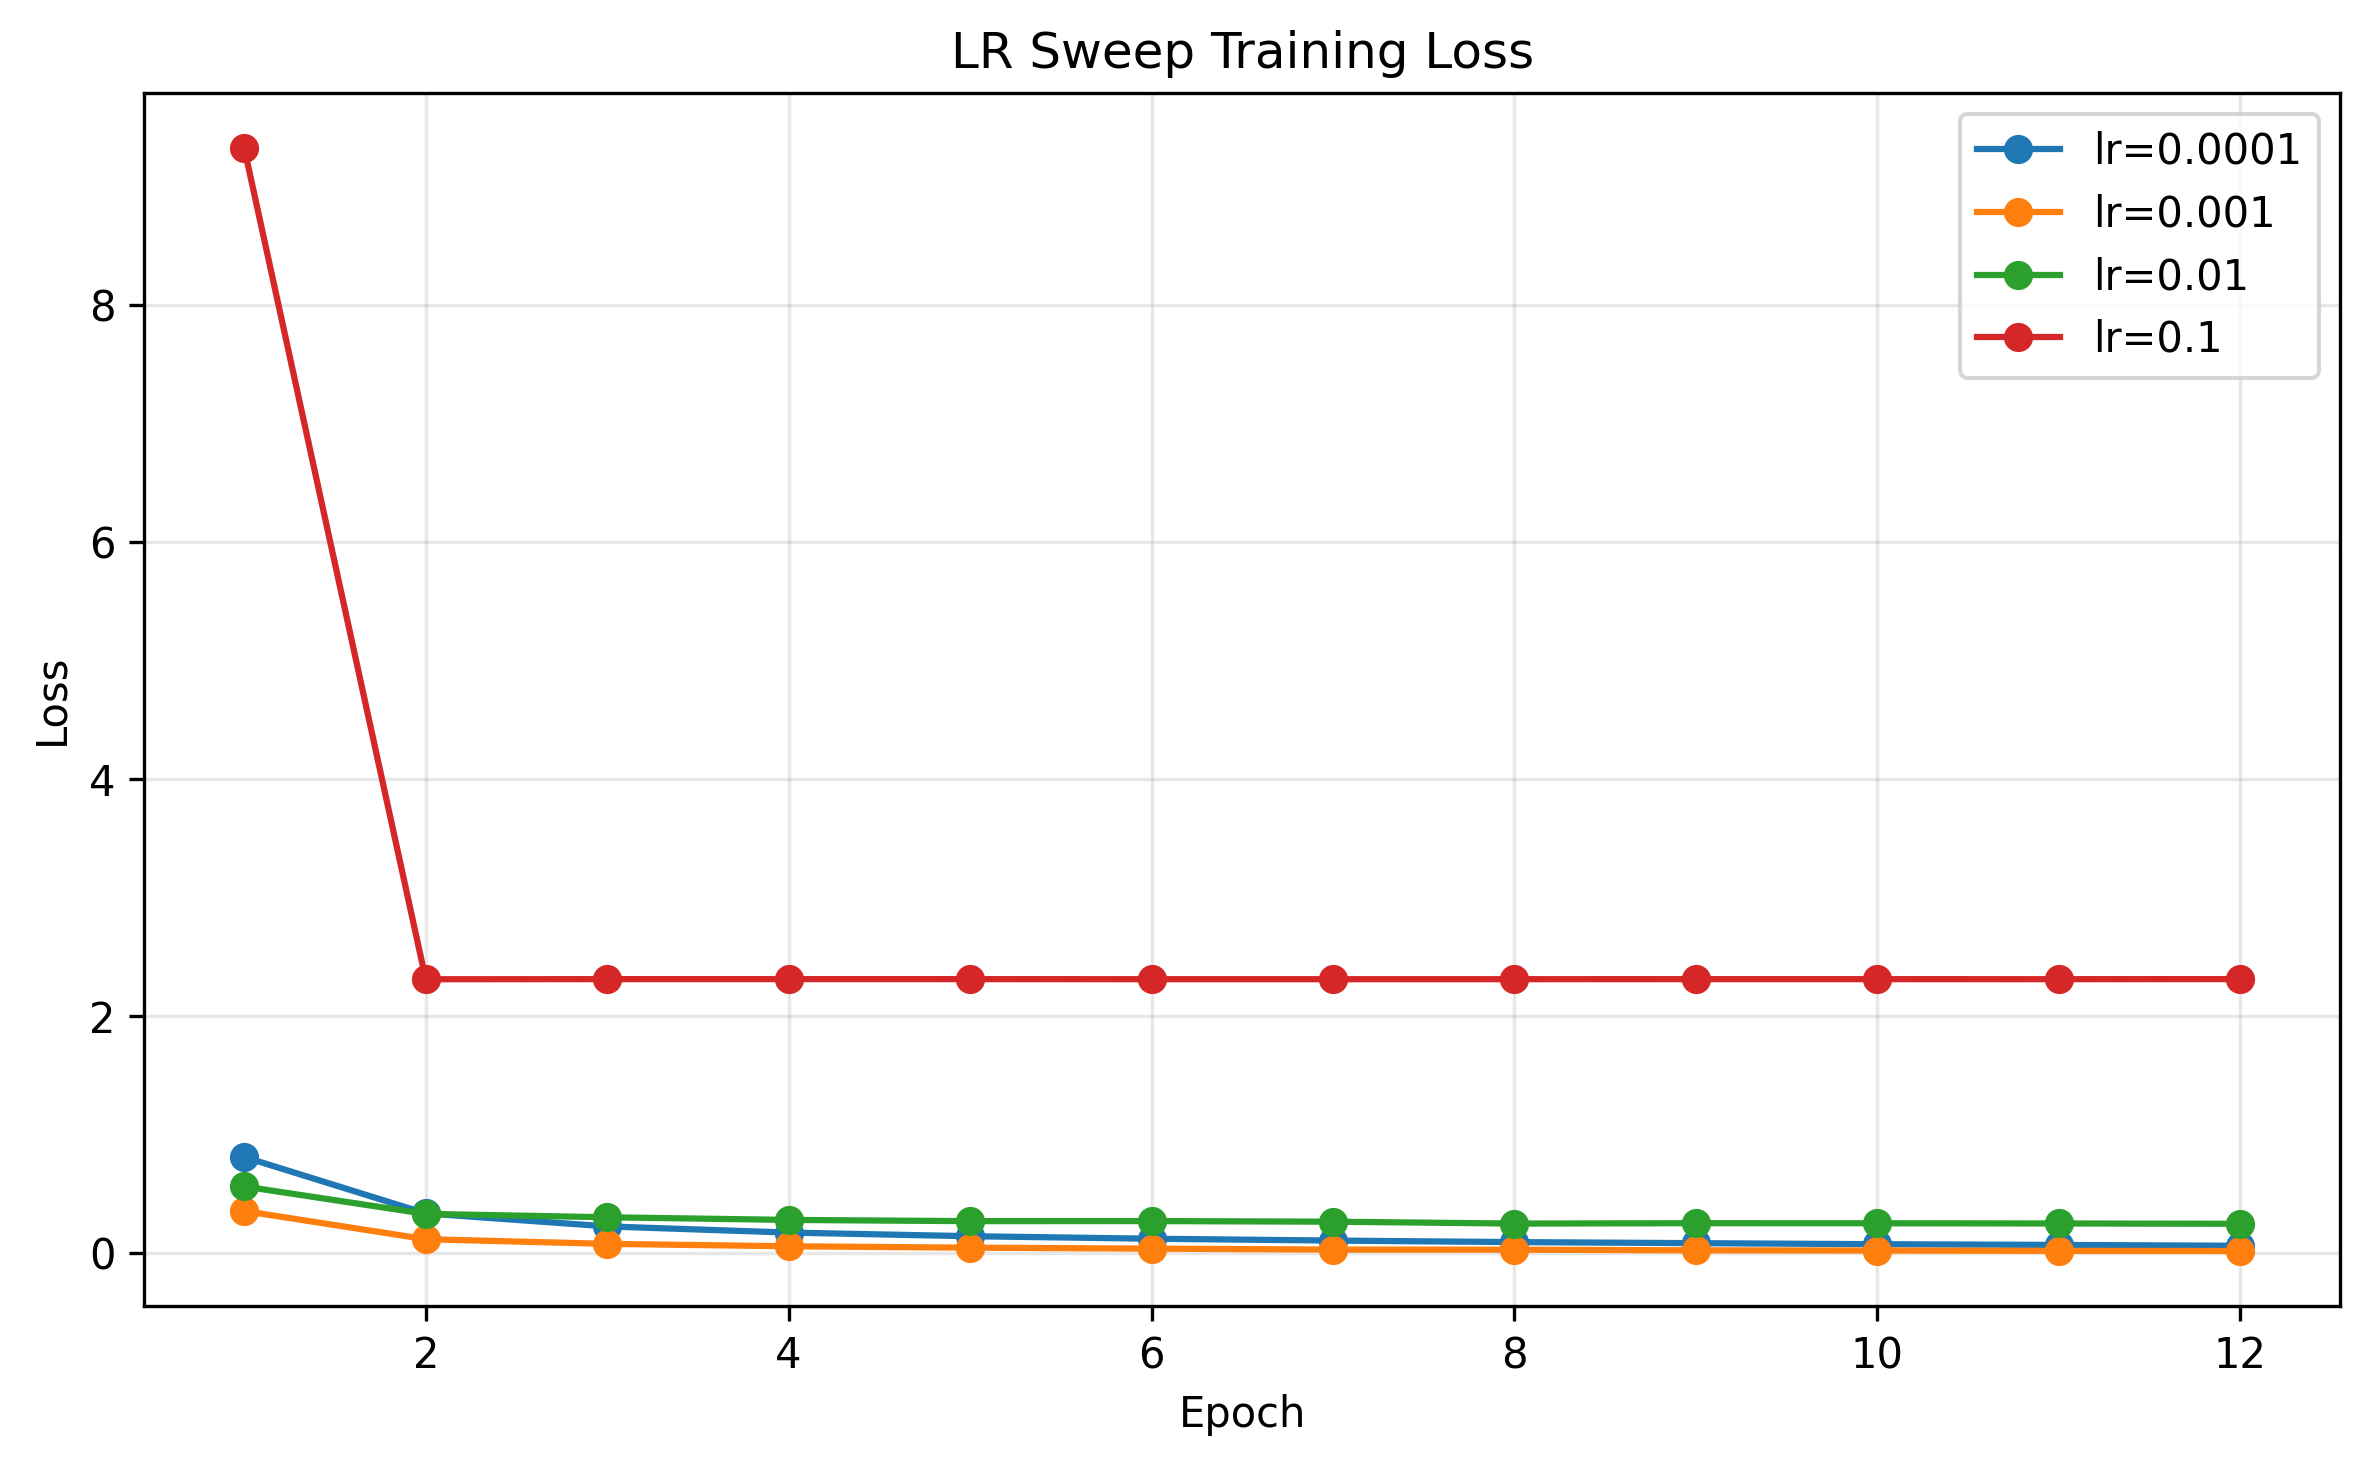
\includegraphics[height=1.46in,keepaspectratio]{figures/lr_comparison_loss.png}
    }
    \hfill
    \subfloat[Training and test accuracy across learning rates.\label{fig:lr_acc}]{
        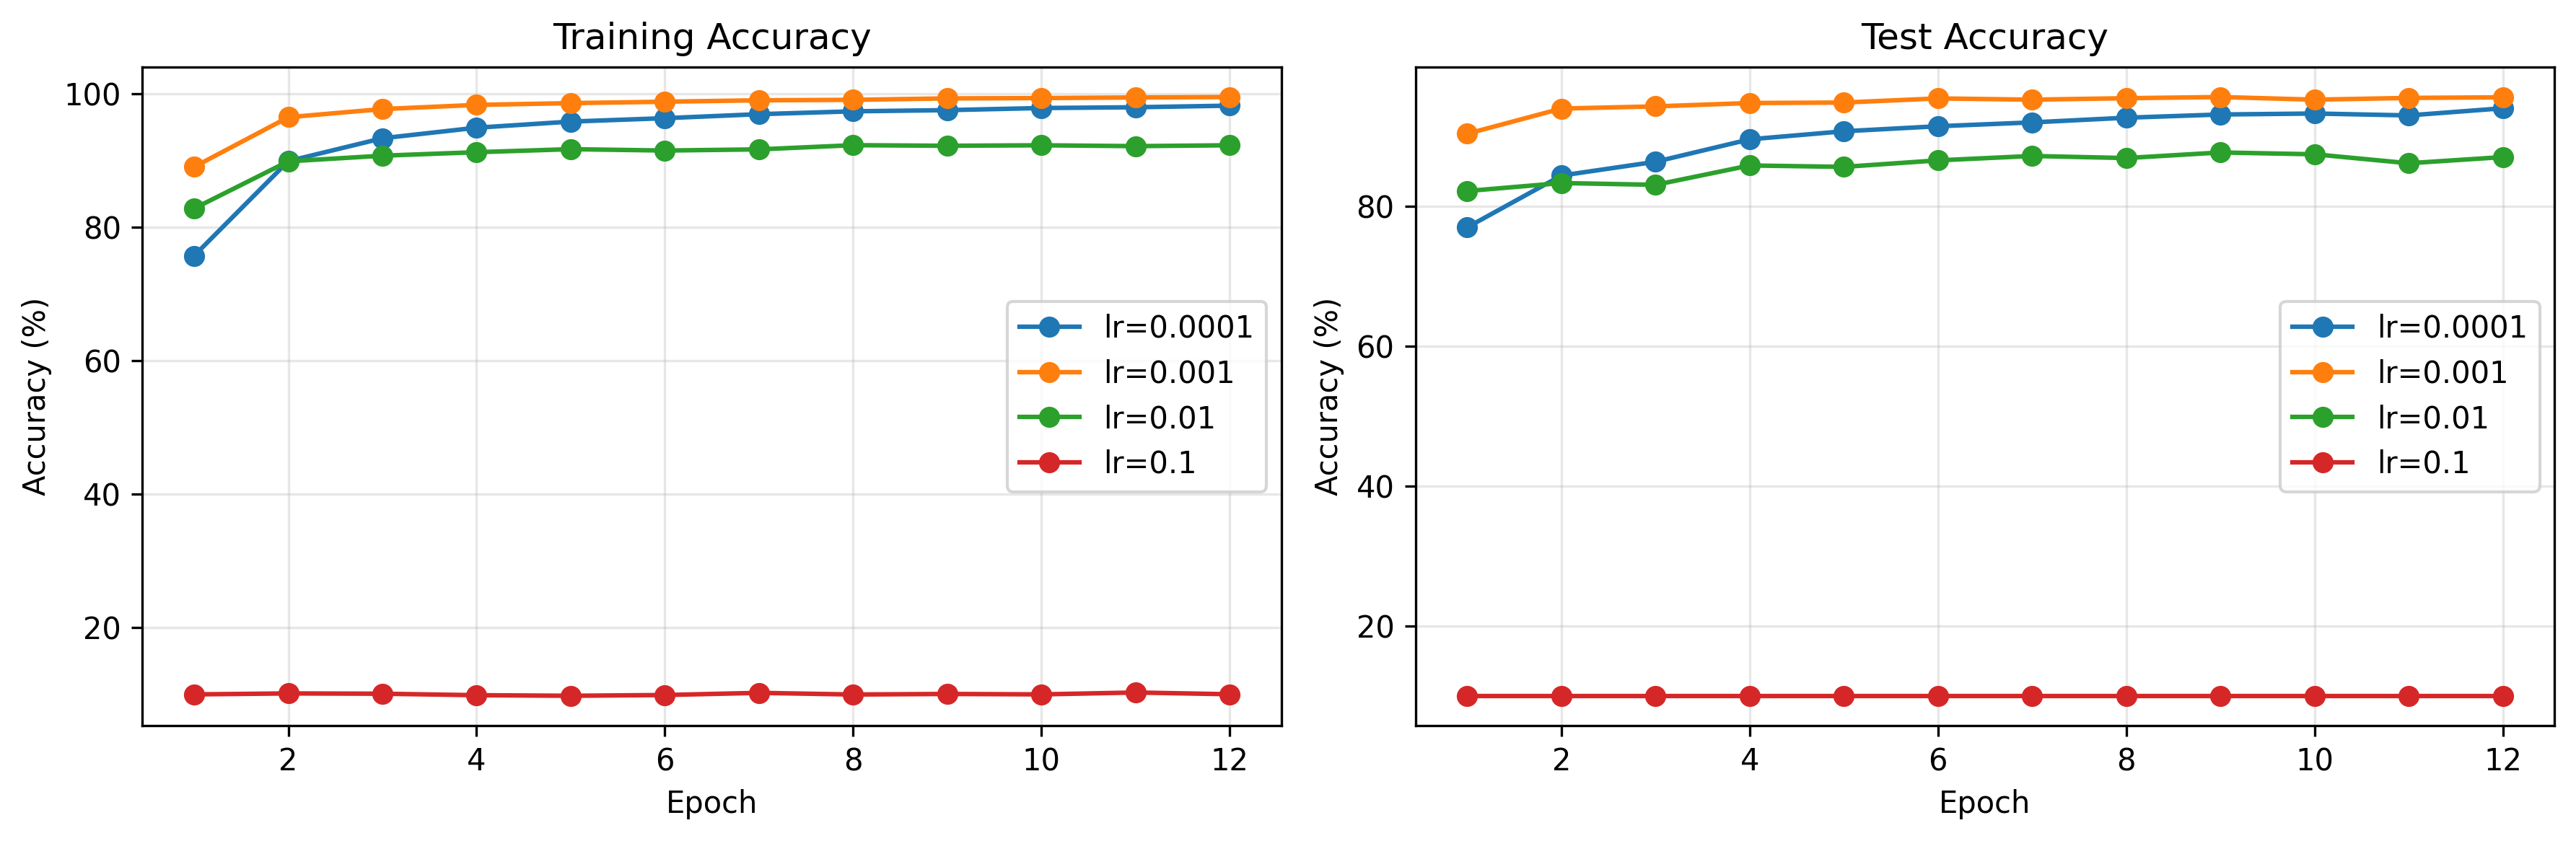
\includegraphics[height=1.46in,keepaspectratio]{figures/lr_comparison_accuracy.png}
    }
    \caption{Learning-rate comparison for the completed KMNIST runs.}
    \label{fig:lr_comparison}
\end{figure*}

\begin{table}[t]
    \centering
    \scriptsize
    \resizebox{\columnwidth}{!}{%
    \begin{tabular}{cccc}
        \toprule
        Learning rate & Best validation acc. & Best test acc. & Final test acc. \\
        \midrule
        0.1 & 10.50\% & 10.00\% & 10.00\% \\
        0.01 & 95.02\% & 87.70\% & 87.04\% \\
        0.001 & 98.60\% & 95.63\% & 95.59\% \\
        0.0001 & 97.92\% & 94.02\% & 94.02\% \\
        \bottomrule
    \end{tabular}
    }
    \caption{Learning-rate sweep results from the saved summary file.}
    \label{tab:lr_sweep}
\end{table}

The value 0.1 failed almost completely. Its test accuracy remained at $10.00\%$, which is effectively chance level for a 10-class classification problem. This indicates that the optimizer steps were too large for stable learning. The value 0.01 learned meaningful structure, but still performed much worse than the best setting, reaching a best test accuracy of only $87.70\%$. By contrast, 0.001 produced the strongest overall performance and therefore justifies its use in the baseline configuration.

The smallest value, 0.0001, also produced a respectable result, but it was clearly weaker than 0.001 within the fixed 12-epoch budget. This pattern is easy to interpret. If the learning rate is too high, the optimizer overshoots useful regions of parameter space; if it is too low, learning becomes unnecessarily slow. Under the conditions of this project, 0.001 provides the best balance between stable optimization and rapid convergence. This is also consistent with the common use of Adam at this scale \cite{kingma2015}.

From a project perspective, the learning-rate comparison demonstrates that optimization choices can matter more than model complexity. The difference between the best and worst learning-rate settings was larger than 85 percentage points in best test accuracy. That is far more consequential than the smaller differences observed in the batch-size sweep.

\subsection{Batch-size comparison}

The batch-size sweep compares the values 8, 16, 32, 64, and 128 while holding the learning rate fixed at 0.001. The corresponding plots are shown in Figure~\ref{fig:batch_comparison}, and the results are summarized in Table~\ref{tab:batch_sweep}.

\begin{figure*}[!t]
    \centering
    \subfloat[Training loss across batch sizes.\label{fig:batch_loss}]{
        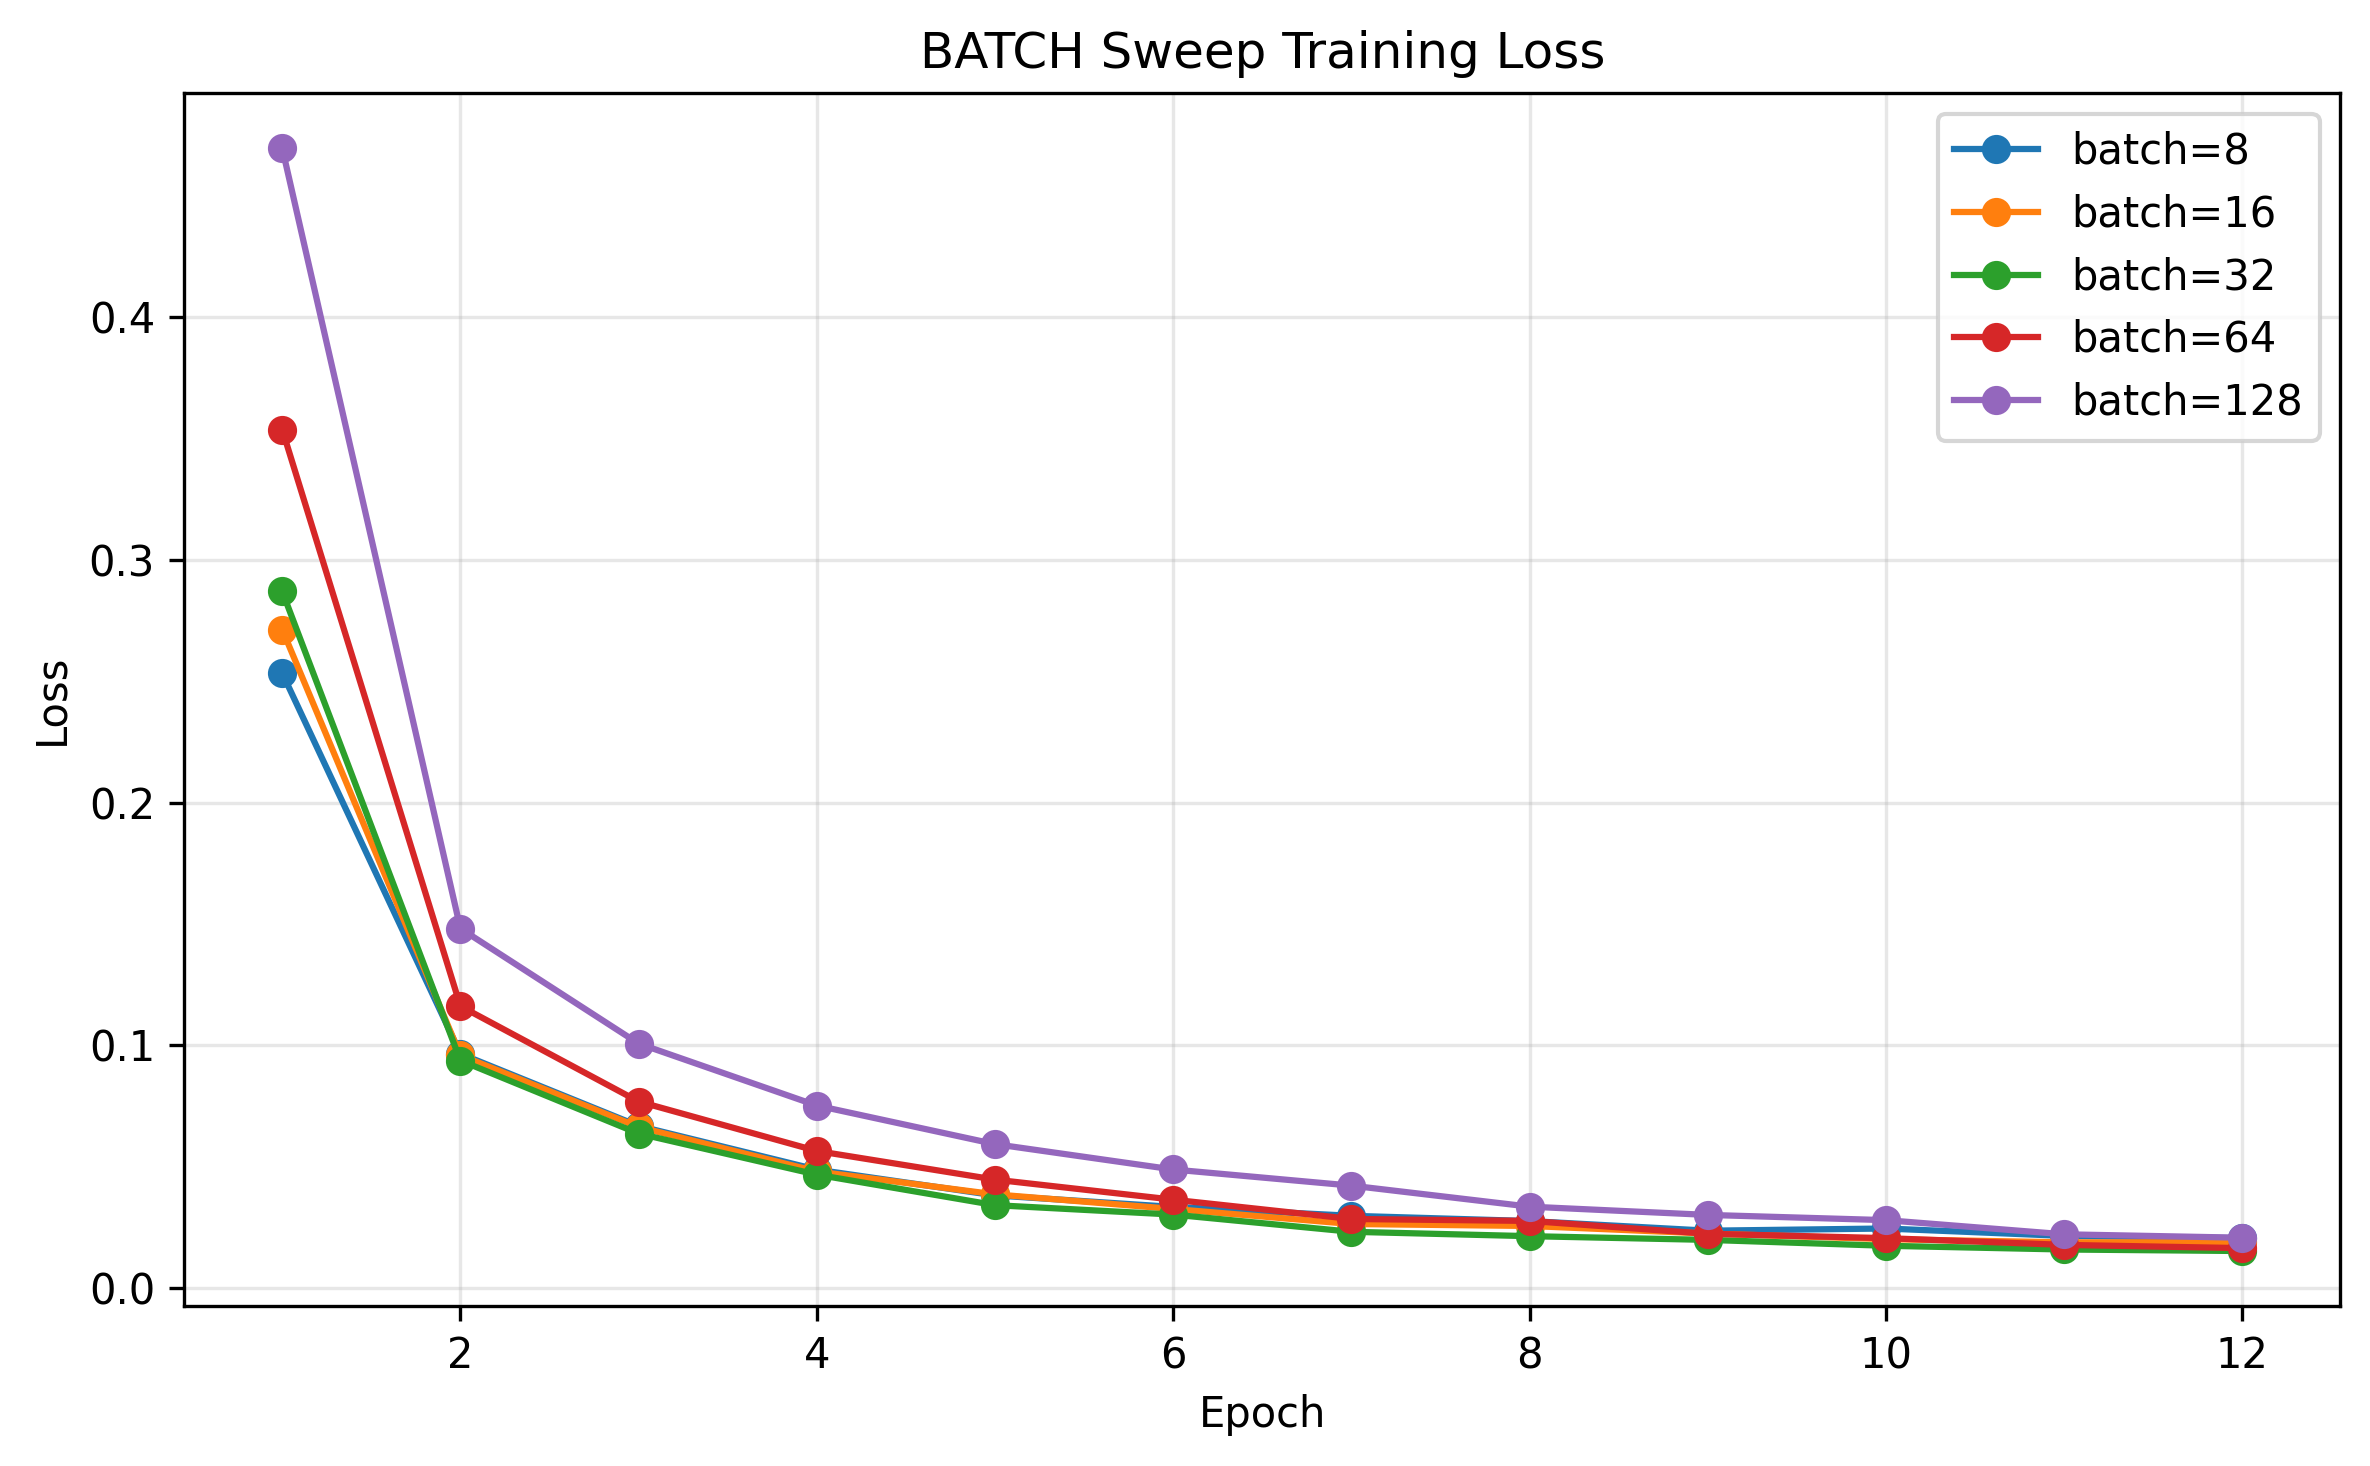
\includegraphics[height=1.46in,keepaspectratio]{figures/batch_comparison_loss.png}
    }
    \hfill
    \subfloat[Training and test accuracy across batch sizes.\label{fig:batch_acc}]{
        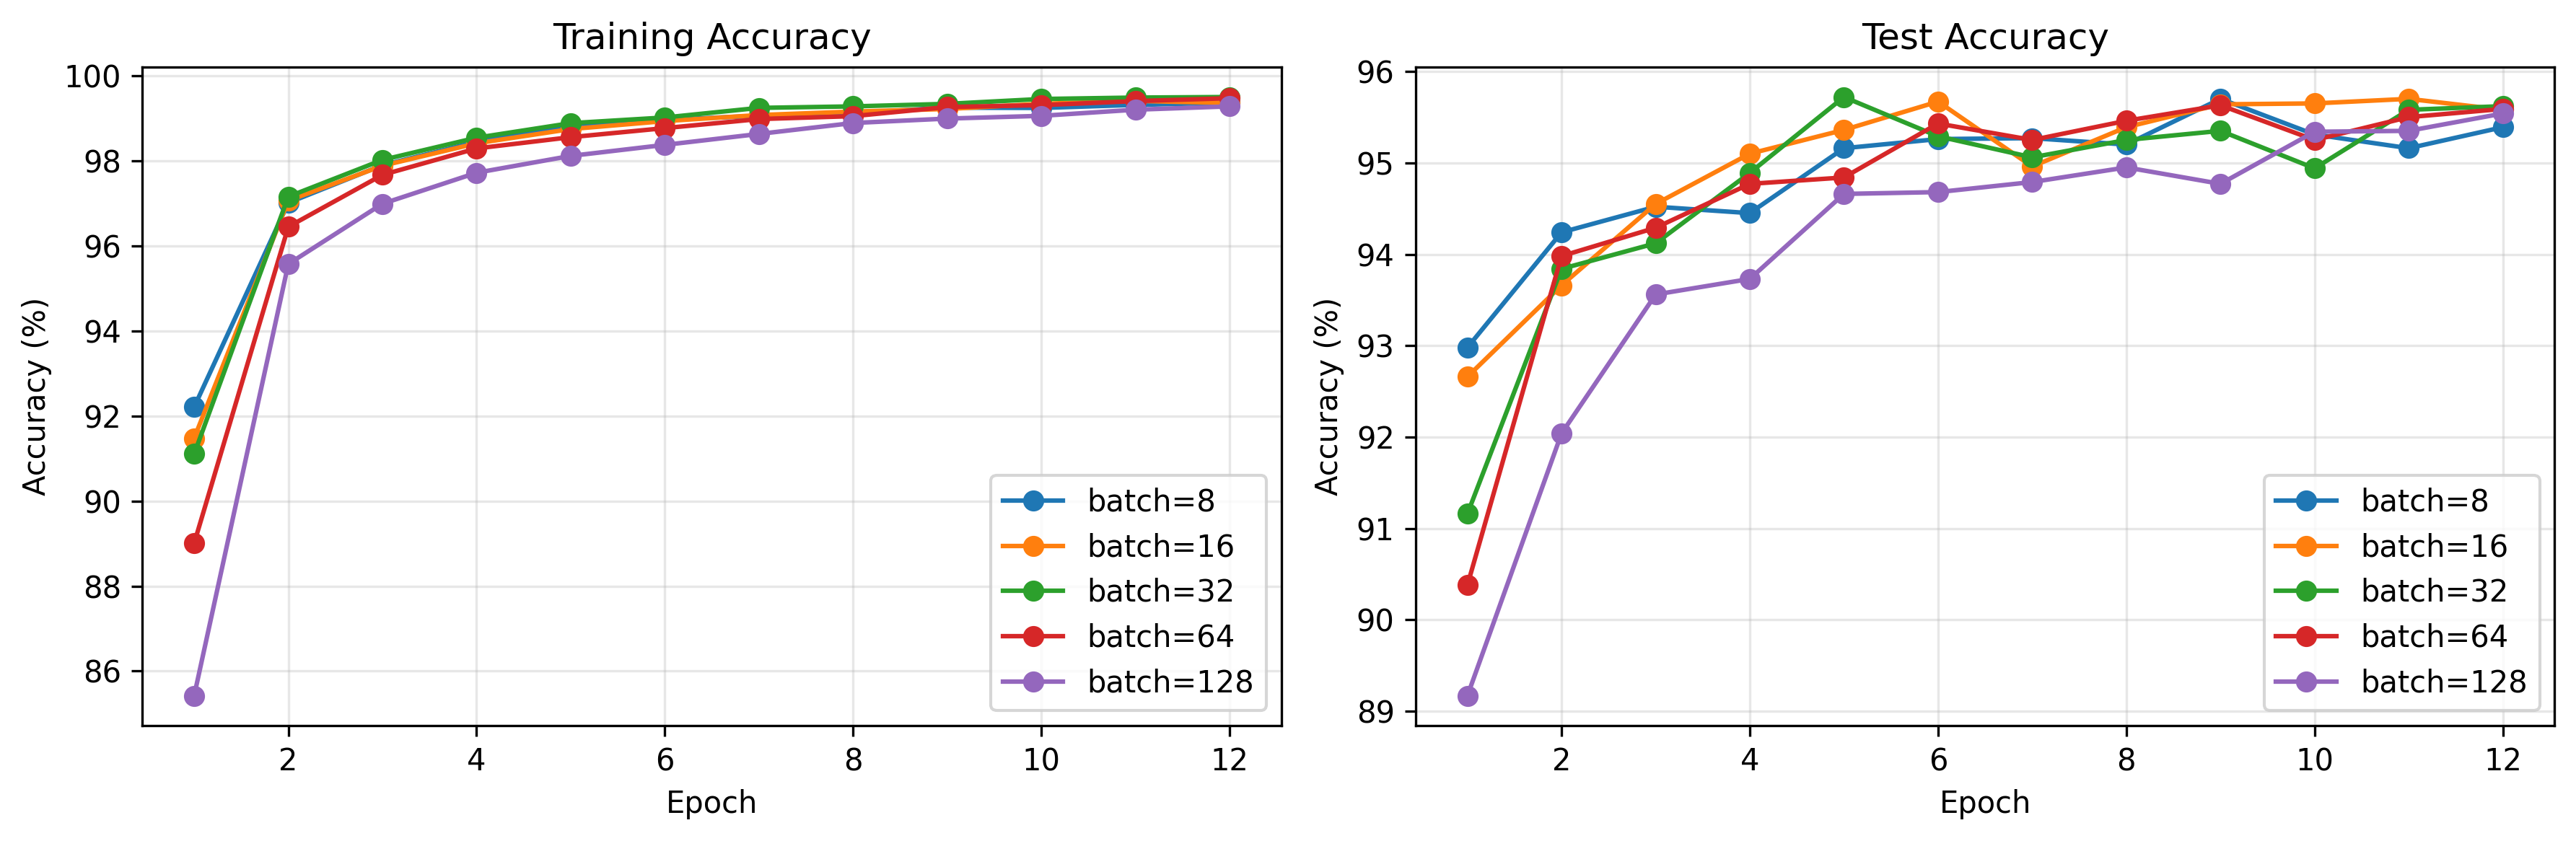
\includegraphics[height=1.46in,keepaspectratio]{figures/batch_comparison_accuracy.png}
    }
    \caption{Batch-size comparison for the completed KMNIST runs.}
    \label{fig:batch_comparison}
\end{figure*}

\begin{table}[t]
    \centering
    \scriptsize
    \resizebox{\columnwidth}{!}{%
    \begin{tabular}{cccc}
        \toprule
        Batch size & Best validation acc. & Best test acc. & Final test acc. \\
        \midrule
        8 & 98.62\% & 95.70\% & 95.39\% \\
        16 & 98.60\% & 95.70\% & 95.58\% \\
        32 & 98.65\% & 95.72\% & 95.62\% \\
        64 & 98.60\% & 95.63\% & 95.59\% \\
        128 & 98.52\% & 95.54\% & 95.54\% \\
        \bottomrule
    \end{tabular}
    }
    \caption{Batch-size sweep results from the saved summary file.}
    \label{tab:batch_sweep}
\end{table}

The most striking feature of this table is how similar the results are. All five batch sizes achieved best test accuracy between $95.54\%$ and $95.72\%$. The highest value was obtained with batch size 32, but the margin over the baseline batch size of 64 was only 0.09 percentage points. This indicates that the CNN is relatively robust to batch-size variation in this problem setting.

This is an important practical result. Because the performance spread is very small, the choice of batch size can be made on operational grounds without seriously affecting model quality. Batch size 64 remains an entirely reasonable baseline because it is standard, efficient, and close to the best observed result. The batch-size sweep therefore complements the learning-rate sweep by showing that not all hyperparameters have equally large effects. In this project, learning rate was decisive, whereas batch size had only a limited influence on final accuracy.

\subsection{Qualitative visualization of the first 100 test predictions}

The final required output is a qualitative visualization of the first 100 test samples together with predicted and true labels. The completed figure is shown in Figure~\ref{fig:first100}. It was generated from the saved baseline checkpoint and presents a grid of KMNIST images where each panel reports the predicted class and the corresponding ground-truth label.

\begin{figure*}[!t]
    \centering
    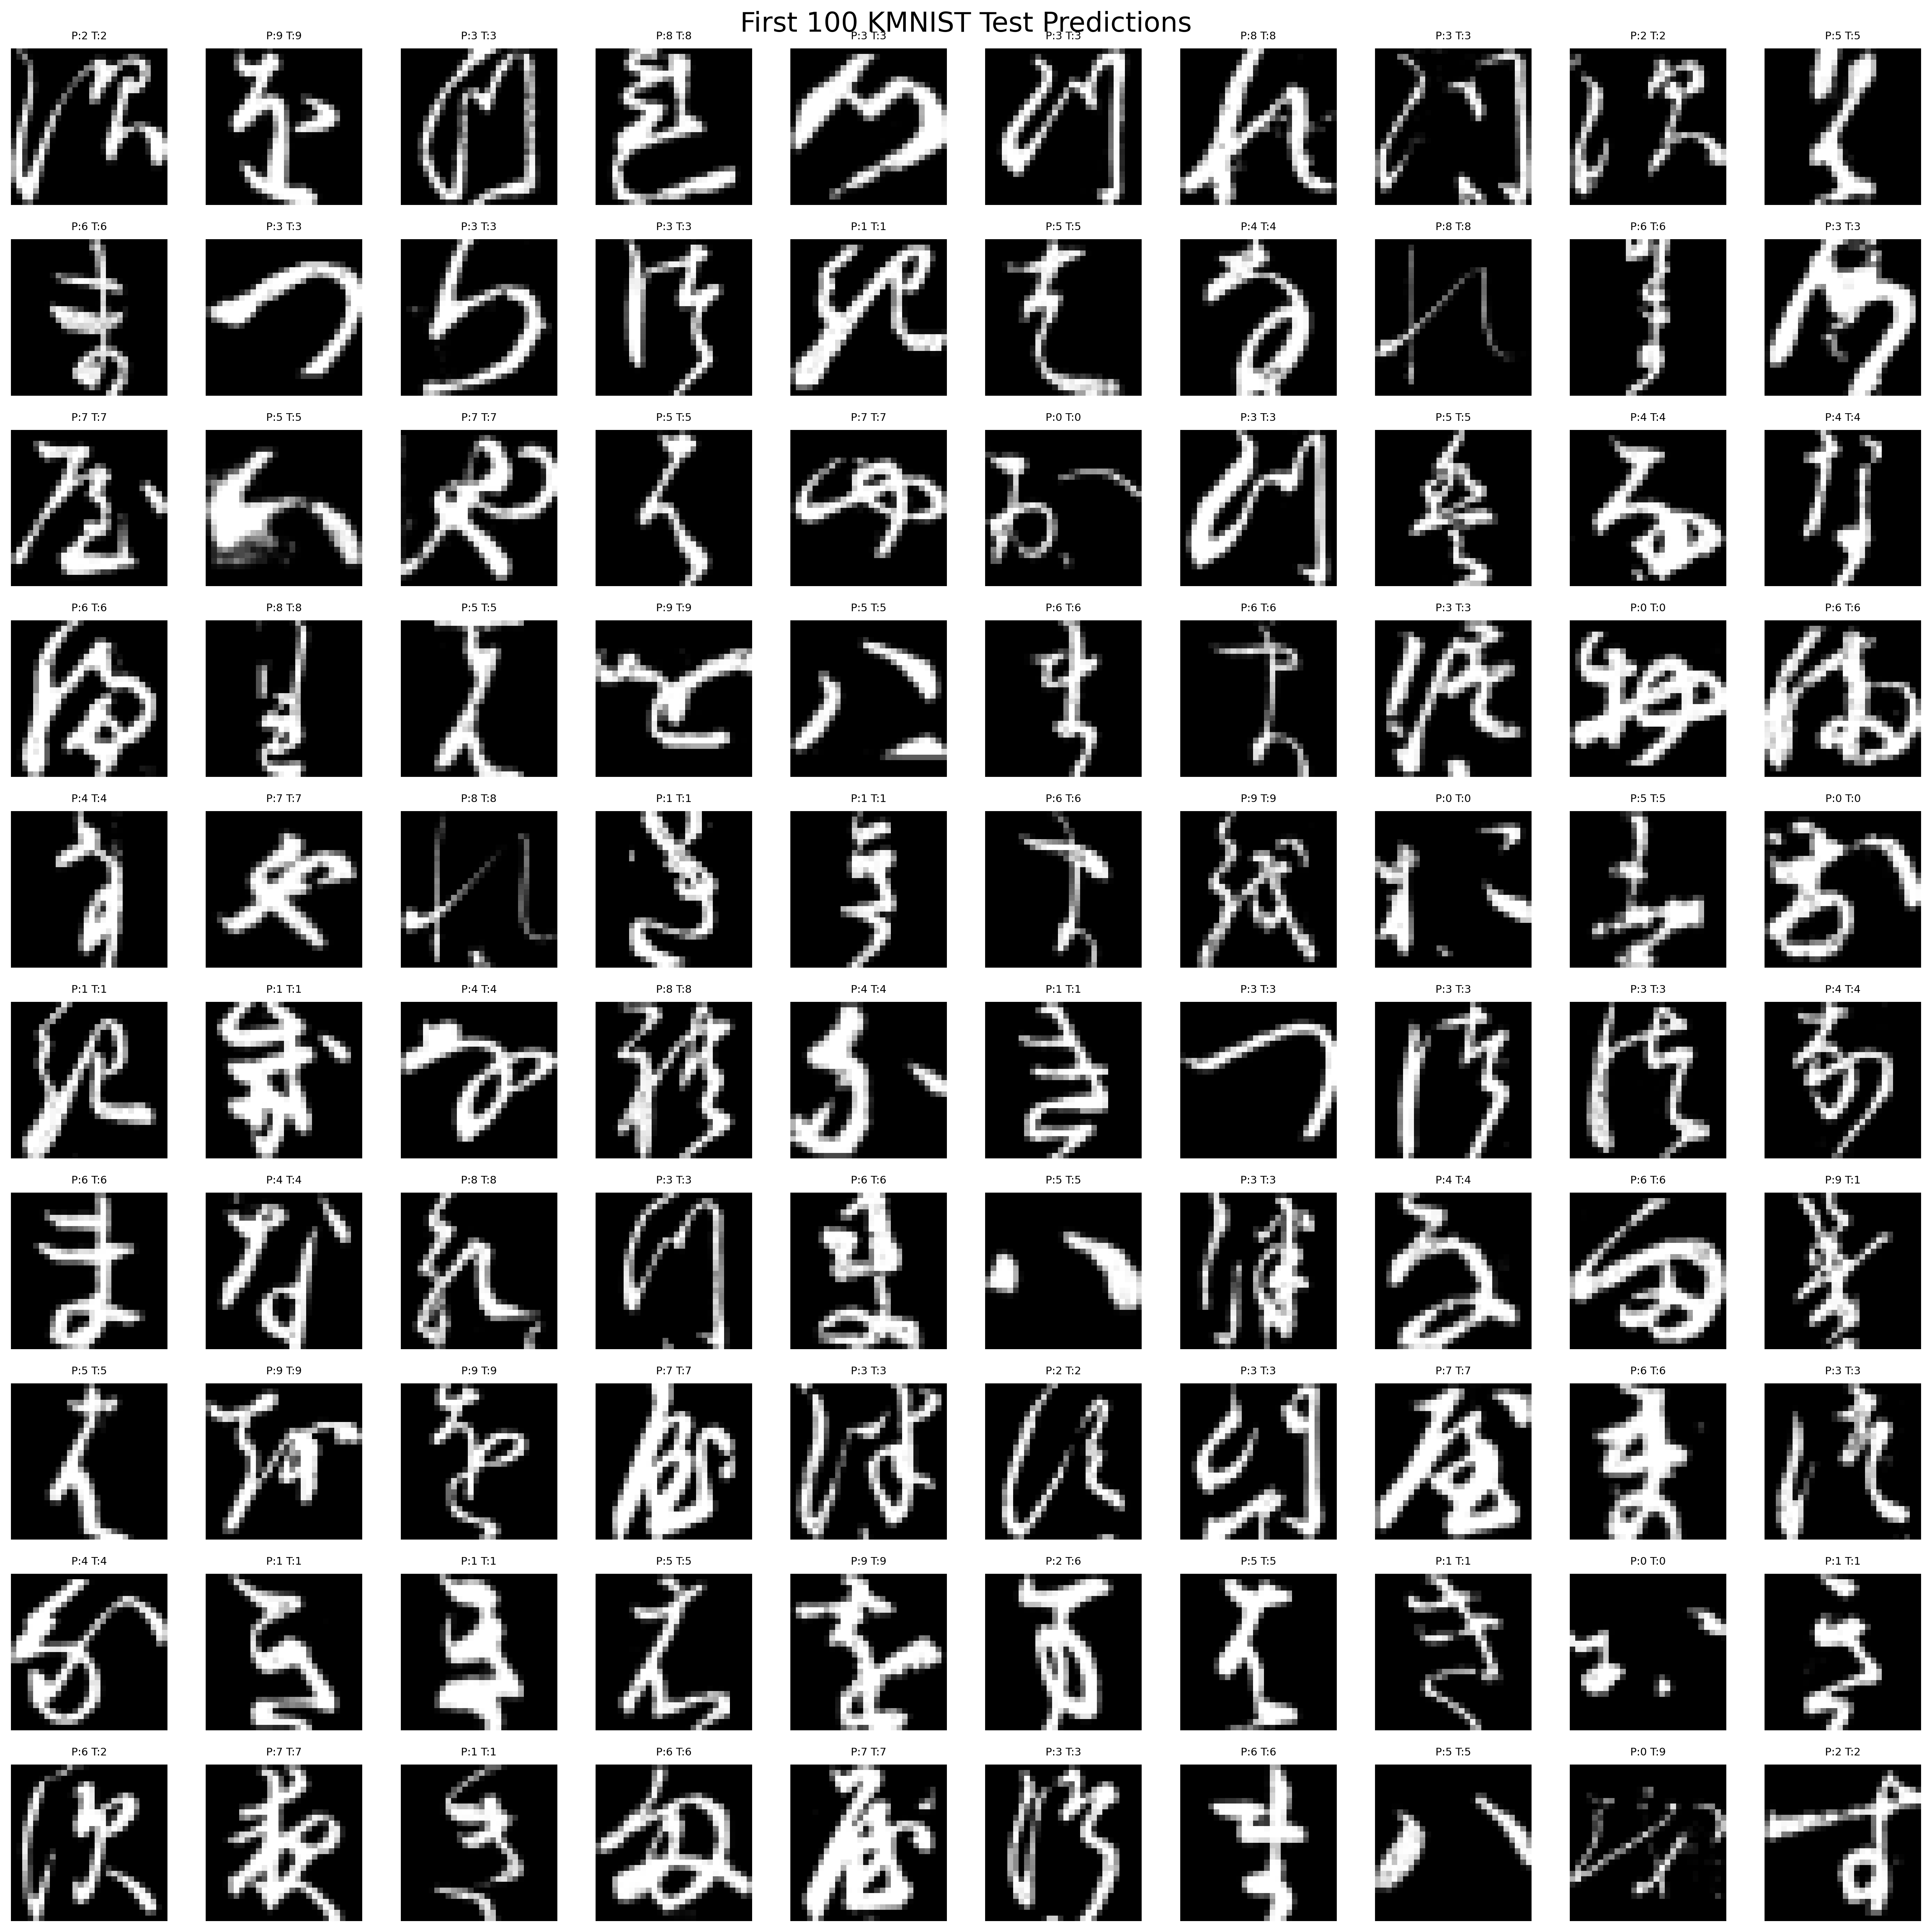
\includegraphics[width=0.72\textwidth,height=5.15in,keepaspectratio]{figures/first_100_test_predictions.png}
    \caption{Visualization of the first 100 test predictions from the saved baseline model. Each image is annotated with the predicted label and the true label.}
    \label{fig:first100}
\end{figure*}

This visualization is useful because it complements the numerical results. Accuracy values summarize overall behavior, but they do not show the character of the model's successes and errors. In the first-100 grid, most predictions are visibly correct, which reinforces the conclusion that the CNN has learned meaningful character features. At the same time, the incorrect cases are also informative because they tend to involve symbols whose stroke patterns are visually similar. This is exactly the type of ambiguity one would expect in a Kuzushiji recognition task.

From the perspective of an academic report, the qualitative figure strengthens the presentation of the results. It demonstrates that the model is not merely achieving a strong aggregate percentage; it is also producing predictions that are visually plausible when inspected sample by sample. This makes the quantitative findings more interpretable for readers who may be less familiar with the raw class labels alone.

\subsection{Overall assessment}

Across all completed experiments, the project demonstrates three main findings. First, a compact CNN is sufficient to achieve strong KMNIST performance, with a baseline best test accuracy of $95.63\%$. Second, a small modification to the loss function improves generalization further, raising the final test accuracy to $96.40\%$. Third, the most influential hyperparameter in the required comparisons was the learning rate, whereas the batch-size effect was comparatively minor.

These findings support the design choices made in the project. The selected model is simple, but not simplistic. The training workflow is concise, but it still includes proper validation-based checkpointing and saved metrics. The experiments are limited to the required comparisons, but they are informative enough to justify the baseline design. As a result, the project satisfies both the technical and explanatory demands of a university deep learning assignment.

\section{Conclusion}

This report has presented a complete KMNIST handwriting-recognition project built with PyTorch and evaluated using the saved outputs in the repository. The work was designed to balance strong predictive performance with clarity of implementation and ease of explanation. That balance is important in academic project work, where a submission must be technically sound, reproducible, and well justified rather than merely complex.

The final baseline system used a two-block convolutional neural network with cross-entropy loss, the Adam optimizer, learning rate 0.001, batch size 64, and 12 epochs of training. Under this configuration, the model achieved a best validation accuracy of $98.60\%$ and a best test accuracy of $95.63\%$. These results confirm that even a relatively small CNN can perform very well on KMNIST when the preprocessing and optimization choices are appropriate.

The comparison experiments added useful depth to the study. Replacing the baseline loss with label-smoothed cross-entropy improved final test accuracy to $96.40\%$, showing that a modest regularization change can improve generalization. The learning-rate sweep demonstrated that 0.001 was clearly the best value among the required settings, while 0.1 failed almost entirely and 0.01 also underperformed substantially. The batch-size sweep showed much smaller variation, with all tested values producing strong results in a narrow accuracy range. Finally, the visualization of the first 100 test predictions provided a qualitative confirmation that the learned model behaves sensibly on individual samples as well as in aggregate metrics.

The project nevertheless has limitations. Only one architecture was implemented, only one random seed was used, and no additional experiments such as data augmentation, confusion-matrix analysis, or learning-rate scheduling were performed. These omissions are acceptable within the scope of the completed work, but they also identify realistic directions for future improvement. If more time were available, the next steps would be to study variability across seeds, inspect class-wise confusion, test lightweight augmentation, and compare the current model against either a simpler multilayer perceptron or a slightly deeper CNN.

Overall, the completed system is a strong and defensible submission. It uses a genuine deep learning approach, provides clear justification for the model and hyperparameters, includes the required performance visualizations, and is supported by saved results that can be traced directly to the repository. The main lesson is that carefully chosen standard methods can be sufficient to produce a high-quality handwriting-recognition system when they are implemented and evaluated rigorously.

\begin{thebibliography}{99}

\bibitem{clanuwat2018}
T. Clanuwat, M. Bober-Irizar, A. Kitamoto, A. Lamb, K. Yamamoto, and D. Ha,
``Deep learning for classical Japanese literature,''
\emph{arXiv preprint arXiv:1812.01718}, 2018.

\bibitem{paszke2019}
A. Paszke, S. Gross, F. Massa, A. Lerer, J. Bradbury, G. Chanan, T. Killeen,
Z. Lin, N. Gimelshein, L. Antiga, A. Desmaison, A. Kopf, E. Yang,
Z. DeVito, M. Raison, A. Tejani, S. Chilamkurthy, B. Steiner, L. Fang,
J. Bai, and S. Chintala,
``PyTorch: An imperative style, high-performance deep learning library,''
in \emph{Advances in Neural Information Processing Systems 32}, 2019,
pp. 8024--8035.

\bibitem{lecun1998}
Y. LeCun, L. Bottou, Y. Bengio, and P. Haffner,
``Gradient-based learning applied to document recognition,''
\emph{Proceedings of the IEEE}, vol. 86, no. 11, pp. 2278--2324, 1998.

\bibitem{goodfellow2016}
I. Goodfellow, Y. Bengio, and A. Courville,
\emph{Deep Learning}.
Cambridge, MA, USA: MIT Press, 2016.

\bibitem{szegedy2016}
C. Szegedy, V. Vanhoucke, S. Ioffe, J. Shlens, and Z. Wojna,
``Rethinking the Inception architecture for computer vision,''
in \emph{Proceedings of the IEEE Conference on Computer Vision and Pattern Recognition}, 2016,
pp. 2818--2826.

\bibitem{kingma2015}
D. P. Kingma and J. Ba,
``Adam: A method for stochastic optimization,''
in \emph{Proceedings of the 3rd International Conference on Learning Representations}, 2015.

\end{thebibliography}

\clearpage
\section*{A. Appendix}

\subsection*{A.1 Team Members}

\begin{center}
\renewcommand{\arraystretch}{1.15}
\footnotesize
\begin{tabular}{@{}p{1.05in}p{0.55in}p{1.30in}@{}}
\toprule
Name & ID & Email \\
\midrule
Mingjianliang* & 5596559 & \url{mingjianliang@ln.hk} \\
Binghechen & 5588057 & \url{binghechen@ln.hk} \\
Yutinghuang & 5537515 & \url{yutinghuang@ln.hk} \\
Hailingu & 5547340 & \url{hailingu@ln.hk} \\
Jiangshanli & 5520354 & \url{jiangshanli@ln.hk} \\
Zhanchunfeng & 5538519 & \url{zhanchunfeng@ln.hk} \\
\bottomrule
\end{tabular}
\end{center}

\noindent * Team leader.

\subsection*{A.2 Contribution Statement}

\noindent Mingjianliang (team leader) was responsible for overall coordination, experimental planning, overall experimental analysis, and final paper integration; Binghechen was responsible for the research and implementation of the core experimental pipeline, including baseline training, experiment organization, and result integration; Yutinghuang was responsible for the research and implementation of the neural network methods, including the baseline convolutional neural network and the main training, validation, and testing workflow; Hailingu was responsible for the research and experiments on the loss-function comparison and learning-rate settings; Jiangshanli was responsible for data investigation, data preprocessing, and support for dataset organization and analysis; Zhanchunfeng was responsible for the research and experiments on batch-size settings, result visualization, and prediction analysis.

\end{document}
